% This LaTeX document needs to be compiled with XeLaTeX.
\documentclass[10pt]{article}
\usepackage[utf8]{inputenc}
\usepackage{graphicx}
\usepackage[export]{adjustbox}
\graphicspath{ {./images/} }
\usepackage{amsmath}
\usepackage{amsfonts}
\usepackage{amssymb}
\usepackage[version=4]{mhchem}
\usepackage{stmaryrd}
\usepackage{multirow}
\usepackage[fallback]{xeCJK}
\usepackage{polyglossia}
\usepackage{fontspec}
\setCJKmainfont{Noto Serif CJK KR}

\setmainlanguage{polish}
\setmainfont{CMU Serif}

\title{WYPEENIA ZDAJACY }

\author{}
\date{}


\begin{document}
\maketitle
\begin{center}

\includegraphics[max width=\textwidth]{2024_11_21_e75cb8afbb07ee23b21bg-01(1)}
\end{center}

\section*{KOD}
PESEL\\
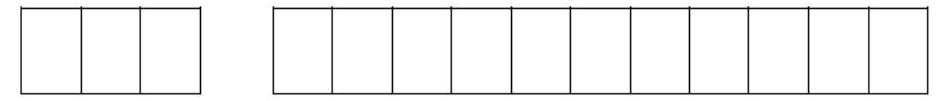
\includegraphics[max width=\textwidth, center]{2024_11_21_e75cb8afbb07ee23b21bg-01}

\section*{Miejsce na naklejkę.}
Sprawdż, czy kod na naklejce to M-100.\\
Jeżeli tak - przyklej naklejkę. Jeżeli nie - zgłoś to nauczycielowi.

\section*{Próbny egzamin maturalny}
\section*{MATEMATYKA}
\section*{POZIOM PODSTAWOWY}
DATA: 15 marca 2023 r. GODZINA ROZPOCZĘCIA: 8:00 CZAS PRACY: 180 minut

\section*{WYPEŁENIA ZESPÓ̌ NADZORUJĄCY}
Uprawnienia zdającego do:\\
dostosowania zasad oceniania dostosowania w zw. z dyskalkulią\\
nieprzenoszenia zaznaczeń na kartę.

\section*{LICZBA PUNKTÓW DO UZYSKANIA: 46}
\section*{Instrukcja dla zdającego}
\begin{enumerate}
  \item Sprawdź, czy arkusz egzaminacyjny zawiera 21 stron (zadania 1-29). Ewentualny brak zgłoś przewodniczącemu zespołu nadzorującego egzamin.
  \item Na pierwszej stronie arkusza oraz na karcie odpowiedzi wpisz swój numer PESEL i przyklej naklejkę z kodem.
  \item Pamiętaj, że pominięcie argumentacji lub istotnych obliczeń w rozwiązaniu zadania otwartego może spowodować, że za to rozwiązanie nie otrzymasz pełnej liczby punktów.
  \item Rozwiązania zadań i odpowiedzi wpisuj w miejscu na to przeznaczonym.
  \item Symbol А в с Damieszczony w nagłówku zadania oznacza, że rozwiązanie zadania zamkniętego musisz przenieść na kartę odpowiedzi.
  \item Odpowiedzi do zadań zamkniętych zaznacz na karcie odpowiedzi w części karty przeznaczonej dla zdającego. Zamaluj pola do tego przeznaczone. Błędne zaznaczenie otocz kółkiem i zaznacz właściwe.
  \item Nie wpisuj żadnych znaków w tabelkach przeznaczonych dla egzaminatora. Tabelki umieszczone są na marginesie przy odpowiednich zadaniach.
  \item Pisz czytelnie i używaj tylko długopisu lub pióra z czarnym tuszem lub atramentem.
  \item Nie używaj korektora, a błędne zapisy wyraźnie przekreśl.
  \item Pamiętaj, że zapisy w brudnopisie nie będą oceniane.
  \item Możesz korzystać z Wybranych wzorów matematycznych, cyrkla i linijki oraz kalkulatora prostego.\\
Życzymy powodzenia!
\end{enumerate}

\section*{Zadanie 1. (0-1) \(\triangle\) в с D}
Dokończ zdanie. Wybierz właściwą odpowiedź spośród podanych.\\
Wartość wyrażenia \(\left(2-2^{-2}\right)^{-1}\) jest równa\\
A. \(\frac{4}{7}\)\\
B. \(1 \frac{3}{4}\)\\
C. \(2 \frac{1}{4}\)\\
D. \(\frac{4}{9}\)

\begin{center}
\begin{tabular}{|c|c|c|c|c|c|c|c|c|c|c|c|c|c|c|c|c|c|c|c|c|c|c|c|c|c|c|}
\hline
\multicolumn{5}{|l|}{Brudnopis} &  &  &  &  &  &  &  &  &  &  &  &  &  &  &  &  &  &  &  &  &  &  \\
\hline
 &  &  &  &  &  &  &  &  &  &  &  &  &  &  &  &  &  &  &  &  &  &  &  &  &  &  \\
\hline
 &  &  &  &  &  &  &  &  &  &  &  &  &  &  &  &  &  &  &  &  &  &  &  &  &  &  \\
\hline
 &  &  &  &  &  &  &  &  &  &  &  &  &  &  &  &  &  &  &  &  &  &  &  &  &  &  \\
\hline
 &  &  &  &  &  &  &  &  &  &  &  &  &  &  &  &  &  &  &  &  &  &  &  &  &  &  \\
\hline
 &  &  &  &  &  &  &  &  &  &  &  &  &  &  &  &  &  &  &  &  &  &  &  &  &  &  \\
\hline
 &  &  &  &  &  &  &  &  &  &  &  &  &  &  &  &  &  &  &  &  &  &  &  &  &  &  \\
\hline
 &  &  &  &  &  &  &  &  &  &  &  &  &  &  &  &  &  &  &  &  &  &  &  &  &  &  \\
\hline
\end{tabular}
\end{center}

Zadanie 2. (0-1) \(\triangle\) в с 미\\
Dokończ zdanie. Wybierz właściwą odpowiedź spośród podanych.\\
Wartość wyrażenia \(\frac{2^{21}+4^{10}+8^{7}}{16^{5}+32^{4}}\) jest równa\\
A. 4\\
B. 1\\
C. \(1 \frac{1}{2}\)\\
D. \(2 \frac{1}{2}\)\\

\includegraphics[max width=\textwidth, center]{2024_11_21_e75cb8afbb07ee23b21bg-02}

\section*{Zadanie 3. (0-1) \(\triangle\) в с D}
Dokończ zdanie. Wybierz właściwą odpowiedź spośród podanych.\\
Wartość wyrażenia \(\log 2 x-3 \log x+\log 5 x^{2}\), gdzie \(x>0\) jest równa\\
A. 4\\
B. 1\\
C. -1\\
D. 2

\begin{center}
\begin{tabular}{|c|c|c|c|c|c|c|c|c|c|c|c|c|c|c|c|c|c|c|c|c|c|c|c|c|c|c|}
\hline
 & Brud & dnop &  &  &  &  &  &  &  &  &  &  &  &  &  &  &  &  &  &  &  &  &  &  &  &  \\
\hline
 &  &  &  &  &  &  &  &  &  &  &  &  &  &  &  &  &  &  &  &  &  &  &  &  &  &  \\
\hline
 &  &  &  &  &  &  &  &  &  &  &  &  &  &  &  &  &  &  &  &  &  &  &  &  &  &  \\
\hline
 &  &  &  &  &  &  &  &  &  &  &  &  &  &  &  &  &  &  &  &  &  &  &  &  &  &  \\
\hline
 &  &  &  &  &  &  &  &  &  &  &  &  &  &  &  &  &  &  &  &  &  &  &  &  &  &  \\
\hline
 &  &  &  &  &  &  &  &  &  &  &  &  &  &  &  &  &  &  &  &  &  &  &  &  &  &  \\
\hline
 &  &  &  &  &  &  &  &  &  &  &  &  &  &  &  &  &  &  &  &  &  &  &  &  &  &  \\
\hline
 &  &  &  &  &  &  &  &  &  &  &  &  &  &  &  &  &  &  &  &  &  &  &  &  &  &  \\
\hline
 &  &  &  &  &  &  &  &  &  &  &  &  &  &  &  &  &  &  &  &  &  &  &  &  &  &  \\
\hline
 &  &  &  &  &  &  &  &  &  &  &  &  &  &  &  &  &  &  &  &  &  &  &  &  &  &  \\
\hline
 &  &  &  &  &  &  &  &  &  &  &  &  &  &  &  &  &  &  &  &  &  &  &  &  &  &  \\
\hline
\end{tabular}
\end{center}

\section*{Zadanie 4. (0-1) \(\triangle\) B C D}
Pan Kowalski wpłacił do banku kwotę 30000 zł. Oprocentowanie wkładu wynosi \(3 \%\) w skali roku. Bank zagwarantował, że oprocentowanie nie zmieni się przez trzy kolejne lata. Odsetki są naliczane i kapitalizowane co rok (nie uwzględniamy podatku od odsetek).

\section*{Dokończ zdanie. Wybierz właściwą odpowiedź spośród podanych.}
Kwota odsetek doliczonych do wkładu ulokowanego przez pana Kowalskiego po trzech latach będzie równa\\
A. 2700 zt\\
B. \(30000 \cdot(1,03)^{3} \mathrm{zł}\)\\
C. \(30000 \cdot(0,03)^{3} \mathrm{zł}\)\\
D. \(2781,81 \mathrm{zt}\)\\

\includegraphics[max width=\textwidth, center]{2024_11_21_e75cb8afbb07ee23b21bg-03}

Zadanie 5. (0-2)\\
Dokończ zdanie. Wybierz dwie właściwe odpowiedzi spośród podanych.\\
Dla każdej liczby rzeczywistej \(x\) i dla każdej liczby rzeczywistej \(y\) wyrażenie \((x-y)^{2}-(2 x+y)^{2}\) jest równe\\
A. \(-3 x(x+2 y)\)\\
B. \(-2 x^{2}+2 y^{2}-4 x y\)\\
C. \((x-y)(x+y)-(2 x+y)(2 x-y)\)\\
D. \((x-y)^{2}+(-2 x-y)^{2}\)\\
E. \(-3 x^{2}-2 y^{2}\)\\
F. \((x-3 y)^{2}-4 x^{2}-9 y^{2}\)\\
G. \(-(y-x)^{2}+(-2 x+y)^{2}\)

\begin{center}
\begin{tabular}{|c|c|c|c|c|c|c|c|c|c|c|c|c|c|c|c|c|c|c|c|c|c|c|c|c|c|c|}
\hline
 & Brudn & dnop &  &  &  &  &  &  &  &  &  &  &  &  &  &  &  &  &  &  &  &  &  &  &  &  \\
\hline
 &  &  &  &  &  &  &  &  &  &  &  &  &  &  &  &  &  &  &  &  &  &  &  &  &  &  \\
\hline
 &  &  &  &  &  &  &  &  &  &  &  &  &  &  &  &  &  &  &  &  &  &  &  &  &  &  \\
\hline
 &  &  &  &  &  &  &  &  &  &  &  &  &  &  &  &  &  &  &  &  &  &  &  &  &  &  \\
\hline
 &  &  &  &  &  &  &  &  &  &  &  &  &  &  &  &  &  &  &  &  &  &  &  &  &  &  \\
\hline
 &  &  &  &  &  &  &  &  &  &  &  &  &  &  &  &  &  &  &  &  &  &  &  &  &  &  \\
\hline
 &  &  &  &  &  &  &  &  &  &  &  &  &  &  &  &  &  &  &  &  &  &  &  &  &  &  \\
\hline
 &  &  &  &  &  &  &  &  &  &  &  &  &  &  &  &  &  &  &  &  &  &  &  &  &  &  \\
\hline
 &  &  &  &  &  &  &  &  &  &  &  &  &  &  &  &  &  &  &  &  &  &  &  &  &  &  \\
\hline
 &  &  &  &  &  &  &  &  &  &  &  &  &  &  &  &  &  &  &  &  &  &  &  &  &  &  \\
\hline
 &  &  &  &  &  &  &  &  &  &  &  &  &  &  &  &  &  &  &  &  &  &  &  &  &  &  \\
\hline
\end{tabular}
\end{center}

\section*{Zadanie 6. (0-1) A в с D}
Liczby \(x\) oraz \(y\) spełniają warunek \(x \neq 2 y\).\\
Dokończ zdanie. Wybierz właściwą odpowiedź spośród podanych.\\
Wyrażenie \(\quad \frac{3}{x-2 y}-2\) można przekształcić do postaci\\
A. \(\frac{1}{x-2 y}\)\\
B. \(\frac{3-2 x-4 y}{x-2 y}\)\\
C. \(\frac{3-2 x-2 y}{x-2 y}\)\\
D. \(\frac{3-2 x+4 y}{x-2 y}\)

\begin{center}
\begin{tabular}{|c|c|c|c|c|c|c|c|c|c|c|c|c|c|c|c|c|c|c|c|c|c|c|c|c|c|c|}
\hline
\multicolumn{5}{|l|}{Brudnopis} &  &  &  &  &  &  &  &  &  &  &  &  &  &  &  &  &  &  &  &  &  &  \\
\hline
 &  &  &  &  &  &  &  &  &  &  &  &  &  &  &  &  &  &  &  &  &  &  &  &  &  &  \\
\hline
 &  &  &  &  &  &  &  &  &  &  &  &  &  &  &  &  &  &  &  &  &  &  &  &  &  &  \\
\hline
 &  &  &  &  &  &  &  &  &  &  &  &  &  &  &  &  &  &  &  &  &  &  &  &  &  &  \\
\hline
 &  &  &  &  &  &  &  &  &  &  &  &  &  &  &  &  &  &  &  &  &  &  &  &  &  &  \\
\hline
 &  &  &  &  &  &  &  &  &  &  &  &  &  &  &  &  &  &  &  &  &  &  &  &  &  &  \\
\hline
 &  &  &  &  &  &  &  &  &  &  &  &  &  &  &  &  &  &  &  &  &  &  &  &  &  &  \\
\hline
 &  &  &  &  &  &  &  &  &  &  &  &  &  &  &  &  &  &  &  &  &  &  &  &  &  &  \\
\hline
 &  &  &  &  &  &  &  &  &  &  &  &  &  &  &  &  &  &  &  &  &  &  &  &  &  &  \\
\hline
 &  &  &  &  &  &  &  &  &  &  &  &  &  &  &  &  &  &  &  &  &  &  &  &  &  &  \\
\hline
 &  &  &  &  &  &  &  &  &  &  &  &  &  &  &  &  &  &  &  &  &  &  &  &  &  &  \\
\hline
\end{tabular}
\end{center}

\section*{Zadanie 7. (0-2)}
0-1-2\\
Wykaż, że dla każdej liczby naturalnej nieparzystej \(n\) wyrażenie \(3 n^{2}+6 n+5\) przy dzieleniu przez 12 daje resztę 2.

\begin{center}
\begin{tabular}{|c|c|c|c|c|c|c|c|c|c|c|c|c|c|c|c|c|c|c|c|c|c|c|c|c|c|c|c|}
\hline
 &  &  &  &  &  &  &  &  &  &  &  &  &  &  &  &  &  &  &  &  &  &  &  &  &  &  &  \\
\hline
 &  &  &  &  &  &  &  &  &  &  &  &  &  &  &  &  &  &  &  &  &  &  &  &  &  &  &  \\
\hline
 &  &  &  &  &  &  &  &  &  &  &  &  &  &  &  &  &  &  &  &  &  &  &  &  &  &  &  \\
\hline
 &  &  &  &  &  &  &  &  &  &  &  &  &  &  &  &  &  &  &  &  &  &  &  &  &  &  &  \\
\hline
 &  &  &  &  &  &  &  &  &  &  &  &  &  &  &  &  &  &  &  &  &  &  &  &  &  &  &  \\
\hline
 &  &  &  &  &  &  &  &  &  &  &  &  &  &  &  &  &  &  &  &  &  &  &  &  &  &  &  \\
\hline
 &  &  &  &  &  &  &  &  &  &  &  &  &  &  &  &  &  &  &  &  &  &  &  &  &  &  &  \\
\hline
 &  &  &  &  &  &  &  &  &  &  &  &  &  &  &  &  &  &  &  &  &  &  &  &  &  &  &  \\
\hline
 &  &  &  &  &  &  &  &  &  &  &  &  &  &  &  &  &  &  &  &  &  &  &  &  &  &  &  \\
\hline
 &  &  &  &  &  &  &  &  &  &  &  &  &  &  &  &  &  &  &  &  &  &  &  &  &  &  &  \\
\hline
 &  &  &  &  &  &  &  &  &  &  &  &  &  &  &  &  &  &  &  &  &  &  &  &  &  &  &  \\
\hline
 &  &  &  &  &  &  &  &  &  &  &  &  &  &  &  &  &  &  &  &  &  &  &  &  &  &  &  \\
\hline
 &  &  &  &  &  &  &  &  &  &  &  &  &  &  &  &  &  &  &  &  &  &  &  &  &  &  &  \\
\hline
 &  &  &  &  &  &  &  &  &  &  &  &  &  &  &  &  &  &  &  &  &  &  &  &  &  &  &  \\
\hline
 &  &  &  &  &  &  &  &  &  &  &  &  &  &  &  &  &  &  &  &  &  &  &  &  &  &  &  \\
\hline
 &  &  &  &  &  &  &  &  &  &  &  &  &  &  &  &  &  &  &  &  &  &  &  &  &  &  &  \\
\hline
 &  &  &  &  &  &  &  &  &  &  &  &  &  &  &  &  &  &  &  &  &  &  &  &  &  &  &  \\
\hline
 &  &  &  &  &  &  &  &  &  &  &  &  &  &  &  &  &  &  &  &  &  &  &  &  &  &  &  \\
\hline
 &  &  &  &  &  &  &  &  &  &  &  &  &  &  &  &  &  &  &  &  &  &  &  &  &  &  &  \\
\hline
 &  &  &  &  &  &  &  &  &  &  &  &  &  &  &  &  &  &  &  &  &  &  &  &  &  &  &  \\
\hline
 &  &  &  &  &  &  &  &  &  &  &  &  &  &  &  &  &  &  &  &  &  &  &  &  &  &  &  \\
\hline
 &  &  &  &  &  &  &  &  &  &  &  &  &  &  &  &  &  &  &  &  &  &  &  &  &  &  &  \\
\hline
 &  &  &  &  &  &  &  &  &  &  &  &  &  &  &  &  &  &  &  &  &  &  &  &  &  &  &  \\
\hline
\end{tabular}
\end{center}

\section*{Zadanie 8. (0-1)}
Dokończ zdanie tak, aby było prawdziwe. Wybierz odpowiedź A, B albo C oraz jej uzasadnienie 1., 2 . albo 3.

Układ równań \(\left\{\begin{array}{l}y=-3 x+2 \\ y=(m-1) x-m\end{array}\right.\) z niewiadomymi \(x\) oraz \(y\) ma nieskończenie wiele rozwiązań dla

\begin{center}
\begin{tabular}{|l|c|c|c|c|}
\hline
A. & \(m=-2\) & \multirow{4}{*}{\begin{tabular}{c}
ponieważ w interpretacji \\
\end{tabular}} & 1. & \begin{tabular}{c}
parę różnych prostych \\
równoległych \\
\end{tabular} \\
B. & \(m=1\) &  & \begin{tabular}{c}
parę prostych \\
przecinających się \\
\end{tabular} &  \\
\cline { 1 - 2 }
C. & \(m=\frac{4}{3}\) &  & 3. & \begin{tabular}{c}
parę prostych \\
pokrywających się \\
\end{tabular} \\
\hline
\end{tabular}
\end{center}

\begin{center}
\begin{tabular}{|c|c|c|c|c|c|c|c|c|c|c|c|c|c|c|c|c|c|c|c|c|c|c|c|}
\hline
\multicolumn{4}{|l|}{Brudnopis} &  &  &  &  &  &  &  &  &  &  &  &  &  &  &  &  &  &  &  &  \\
\hline
 &  &  &  &  &  &  &  &  &  &  &  &  &  &  &  &  &  &  &  &  &  &  &  \\
\hline
 &  &  &  &  &  &  &  &  &  &  &  &  &  &  &  &  &  &  &  &  &  &  &  \\
\hline
 &  &  &  &  &  &  &  &  &  &  &  &  &  &  &  &  &  &  &  &  &  &  &  \\
\hline
 &  &  &  &  &  &  &  &  &  &  &  &  &  &  &  &  &  &  &  &  &  &  &  \\
\hline
 &  &  &  &  &  &  &  &  &  &  &  &  &  &  &  &  &  &  &  &  &  &  &  \\
\hline
 &  &  &  &  &  &  &  &  &  &  &  &  &  &  &  &  &  &  &  &  &  &  &  \\
\hline
 &  &  &  &  &  &  &  &  &  &  &  &  &  &  &  &  &  &  &  &  &  &  &  \\
\hline
 &  &  &  &  &  &  &  &  &  &  &  &  &  &  &  &  &  &  &  &  &  &  &  \\
\hline
 &  &  &  &  &  &  &  &  &  &  &  &  &  &  &  &  &  &  &  &  &  &  &  \\
\hline
 &  &  &  &  &  &  &  &  &  &  &  &  &  &  &  &  &  &  &  &  &  &  &  \\
\hline
\end{tabular}
\end{center}

\section*{Zadanie 9. (0-1) \(\triangle \mathrm{BCCO}\)}
Dana jest nierówność

\[
3-\frac{x-3}{2} \geq \frac{x+3}{5}-1
\]

Dokończ zdanie. Wybierz wlaściwą odpowiedź spośród podanych.\\
Najmniejszą liczbą całkowitą, która nie spełnia tej nierówności, jest\\
A. 5\\
B. 7\\
C. 8\\
D. 4\\

\includegraphics[max width=\textwidth, center]{2024_11_21_e75cb8afbb07ee23b21bg-05}

\section*{Zadanie 10. (0-1) \(\triangle\) в с}
Punkty \(A, B, C, D\) leżą na okręgu o środku w punkcie \(S\). Odcinek \(A B\) jest średnicą tego okręgu. Miara kąta \(A B C\) jest równa \(40^{\circ}\) (zobacz rysunek).

\section*{Dokończ zdanie.}
\section*{Wybierz właściwą odpowiedź spośród podanych.}
Miara kąta \(B D C\) jest równa\\
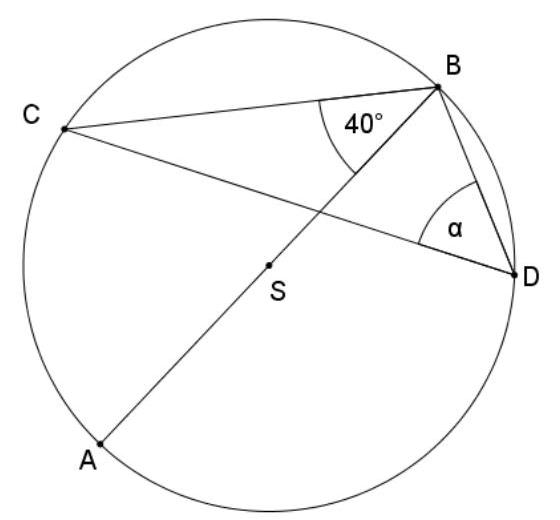
\includegraphics[max width=\textwidth, center]{2024_11_21_e75cb8afbb07ee23b21bg-06}\\
A. \(50^{0}\)\\
B. \(40^{0}\)\\
C. \(45^{0}\)\\
D. \(55^{\circ}\)\\

\includegraphics[max width=\textwidth, center]{2024_11_21_e75cb8afbb07ee23b21bg-06(2)}

\section*{Zadanie 11.}
W kartezjańskim układzie współrzędnych \((x, y)\) przedstawiono fragment wykresu funkcji kwadratowej \(f(x)=a x^{2}+b x+c\). Wierzchołek paraboli, która jest wykresem funkcji \(f\), ma współrzędne \((-3,8)\). Parabola ta przecina oś OX w punktach \((-7,0)\) oraz \((1,0)\).\\
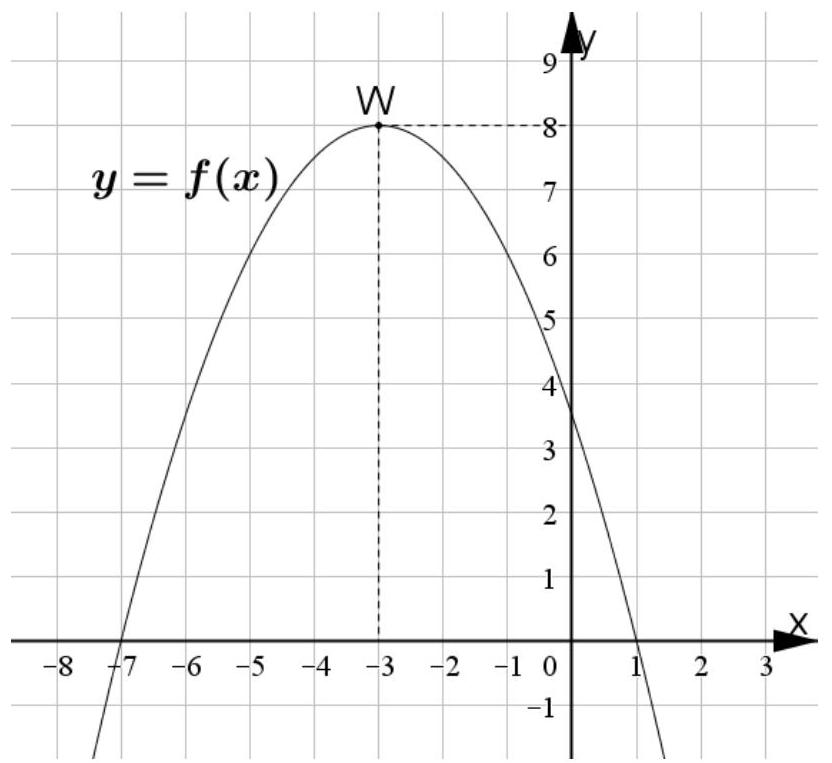
\includegraphics[max width=\textwidth, center]{2024_11_21_e75cb8afbb07ee23b21bg-06(1)}

Zadanie 11.1. (0-1) \(\triangle\)\\
Oceń prawdziwość poniższych stwierdzeń. Zaznacz P, jeśli stwierdzenie jest prawdziwe, albo \(F\) - jeśli jest falszywe.

\begin{center}
\begin{tabular}{|c|l|c|c|}
\hline
1. & Przedział \((-\infty ; 8]\) jest maksymalnym zbiorem, w którym funkcja \(f\) jest rosnąca. & \(\mathbf{P}\) & \(\mathbf{F}\) \\
\hline
2. & Współczynnik \(c\) we wzorze funkcji \(f\) jest liczbą dodatnią. & \(\mathbf{P}\) & \(\mathbf{F}\) \\
\hline
\end{tabular}
\end{center}

\begin{center}
\begin{tabular}{|c|c|c|c|c|c|c|c|c|c|c|c|c|c|c|c|c|c|c|c|c|c|c|c|c|c|}
\hline
\multicolumn{5}{|l|}{Brudnopis} &  &  &  &  &  &  &  &  &  &  &  &  &  &  &  &  &  &  &  &  &  \\
\hline
 &  &  &  &  &  &  &  &  &  &  &  &  &  &  &  &  &  &  &  &  &  &  &  &  &  \\
\hline
 &  &  &  &  &  &  &  &  &  &  &  &  &  &  &  &  &  &  &  &  &  &  &  &  &  \\
\hline
 &  &  &  &  &  &  &  &  &  &  &  &  &  &  &  &  &  &  &  &  &  &  &  &  &  \\
\hline
 &  &  &  &  &  &  &  &  &  &  &  &  &  &  &  &  &  &  &  &  &  &  &  &  &  \\
\hline
 &  &  &  &  &  &  &  &  &  &  &  &  &  &  &  &  &  &  &  &  &  &  &  &  &  \\
\hline
 &  &  &  &  &  &  &  &  &  &  &  &  &  &  &  &  &  &  &  &  &  &  &  &  &  \\
\hline
\end{tabular}
\end{center}

\section*{Zadanie 11.2. (0-1)}
0-1\\
Zapisz poniżej zbiór wszystkich wartości m, dla których nierówność \(f(x)>m\) nie ma rozwiązań.

\section*{Brudnopis}
\subsection*{11.3 Zadanie 11.3. (0-2)}
0-1-2\\
Wyznacz wzór funkcji kwadratowej \(f\) w postaci iloczynowej.\\
Zapisz obliczenia\\

\includegraphics[max width=\textwidth, center]{2024_11_21_e75cb8afbb07ee23b21bg-07}

\section*{Zadanie 12. (0-1) \(\triangle\) в с}
Dany jest wielomian \(W\) określony wzorem \(W(x)=x^{3}+5 x^{2}-3 x-15\) dla każdej liczby rzeczywistej \(x\).

\section*{Dokończ zdanie. Wybierz właściwą odpowiedź spośród podanych.}
Miejscami zerowymi wielomianu \(W\) są liczby\\
A. \(-5,3\)\\
B. \(5,-\sqrt{3}\)\\
C. \(-5, \sqrt{3},-\sqrt{3}\)\\
D. \(5, \sqrt{3},-\sqrt{3}\)

\begin{center}
\begin{tabular}{|c|c|c|c|c|c|c|c|c|c|c|c|c|c|c|c|c|c|c|c|c|c|c|c|c|c|c|}
\hline
\multicolumn{5}{|l|}{Brudnopis} &  &  &  &  &  &  &  &  &  &  &  &  &  &  &  &  &  &  &  &  &  &  \\
\hline
 &  &  &  &  &  &  &  &  &  &  &  &  &  &  &  &  &  &  &  &  &  &  &  &  &  &  \\
\hline
 &  &  &  &  &  &  &  &  &  &  &  &  &  &  &  &  &  &  &  &  &  &  &  &  &  &  \\
\hline
 &  &  &  &  &  &  &  &  &  &  &  &  &  &  &  &  &  &  &  &  &  &  &  &  &  &  \\
\hline
 &  &  &  &  &  &  &  &  &  &  &  &  &  &  &  &  &  &  &  &  &  &  &  &  &  &  \\
\hline
 &  &  &  &  &  &  &  &  &  &  &  &  &  &  &  &  &  &  &  &  &  &  &  &  &  &  \\
\hline
 &  &  &  &  &  &  &  &  &  &  &  &  &  &  &  &  &  &  &  &  &  &  &  &  &  &  \\
\hline
 &  &  &  &  &  &  &  &  &  &  &  &  &  &  &  &  &  &  &  &  &  &  &  &  &  &  \\
\hline
 &  &  &  &  &  &  &  &  &  &  &  &  &  &  &  &  &  &  &  &  &  &  &  &  &  &  \\
\hline
 &  &  &  &  &  &  &  &  &  &  &  &  &  &  &  &  &  &  &  &  &  &  &  &  &  &  \\
\hline
 &  &  &  &  &  &  &  &  &  &  &  &  &  &  &  &  &  &  &  &  &  &  &  &  &  &  \\
\hline
\end{tabular}
\end{center}

\section*{Zadanie 13. (0-1) А в с D}
Dokończ zdanie. Wybierz właściwą odpowiedź spośród podanych.\\
Iloczyn wszystkich rzeczywistych rozwiązań równania \(\frac{(x+3)(2 x-1)\left(x+\frac{2}{3}\right)}{(6 x+4)\left(x+\frac{1}{2}\right)}=0\) jest równy\\
A. 1\\
B. -3\\
C. \(\frac{3}{2}\)\\
D. \(-1 \frac{1}{2}\)

\begin{center}
\begin{tabular}{|c|c|c|c|c|c|c|c|c|c|c|c|c|c|c|c|c|c|c|c|c|c|c|c|c|c|}
\hline
\multicolumn{4}{|l|}{Brudnopis} &  &  &  &  &  &  &  &  &  &  &  &  &  &  &  &  &  &  &  &  &  &  \\
\hline
 &  & 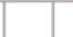
\includegraphics[max width=\textwidth]{2024_11_21_e75cb8afbb07ee23b21bg-08}
 &  &  &  &  &  &  &  &  &  &  &  &  &  &  &  &  &  &  &  &  &  &  &  \\
\hline
 &  &  &  &  &  &  &  &  &  &  &  &  &  &  &  &  &  &  &  &  &  &  &  &  &  \\
\hline
 &  &  &  &  &  &  &  &  &  &  &  &  &  &  &  &  &  &  &  &  &  &  &  &  &  \\
\hline
 &  &  &  &  &  &  &  &  &  &  &  &  &  &  &  &  &  &  &  &  &  &  &  &  &  \\
\hline
 &  &  &  &  &  &  &  &  &  &  &  &  &  &  &  &  &  &  &  &  &  &  &  &  &  \\
\hline
 &  &  &  &  &  &  &  &  &  &  &  &  &  &  &  &  &  &  &  &  &  &  &  &  &  \\
\hline
 &  &  &  &  &  &  &  &  &  &  &  &  &  &  &  &  &  &  &  &  &  &  &  &  &  \\
\hline
 &  &  &  &  &  &  &  &  &  &  &  &  &  &  &  &  &  &  &  &  &  &  &  &  &  \\
\hline
 &  &  &  &  &  &  &  &  &  &  &  &  &  &  &  &  &  &  &  &  &  &  &  &  &  \\
\hline
 &  &  &  &  &  &  &  &  &  &  &  &  &  &  &  &  &  &  &  &  &  &  &  &  &  \\
\hline
\end{tabular}
\end{center}

Dany jest ciąg arytmetyczny \(\left(a_{n}\right)\), określony dla każdej liczby naturalnej \(n \geq 1\).\\
W tym ciągu \(a_{3}=5, a_{3}+a_{4}=13\).\\
Dokończ zdanie. Zaznacz dwie odpowiedzi tak, aby dla każdej z nich dokończenie poniższego zdania było prawdziwe.

Wzór ogólny ciągu \(\left(a_{n}\right)\) może mieć postać\\
A. \(a_{n}=2 n+1\)\\
B. \(a_{n}=\frac{3 n^{2}+2 n-8}{n+2}\)\\
C. \(a_{n}=(n+4)(2 n-1)\)\\
D. \(a_{n}=3 n-4\)\\
E. \(a_{n}=8 n-19\)\\
F. \(a_{n}=n^{2}-4\)\\
G. \(a_{n}=2^{n}-3\)\\

\includegraphics[max width=\textwidth, center]{2024_11_21_e75cb8afbb07ee23b21bg-09}

Zadanie 15. (0-1) A B с D\\
Czterowyrazowy ciąg ( \(-2,3, x, y\) ) jest geometryczny.

\section*{Dokończ zdanie. Wybierz właściwą odpowiedź spośród podanych.}
Liczby \(x\) oraz \(y\) są równe\\
A. \(x=8\) oraz \(y=13\)\\
B. \(x=-2\) oraz \(y=\frac{4}{3}\)\\
C. \(x=-15\) oraz \(y=45\)\\
D. \(x=-4,5\) oraz \(y=6,75\)\\

\includegraphics[max width=\textwidth, center]{2024_11_21_e75cb8afbb07ee23b21bg-09(1)}

\section*{Zadanie 16.}
W kartezjańskim układzie współrzędnych \((x, y)\) przedstawiono wykres funkcji \(y=f(x)\) określonej dla każdej liczby rzeczywistej \(x\) należącej do przedziału (0; 9].\\
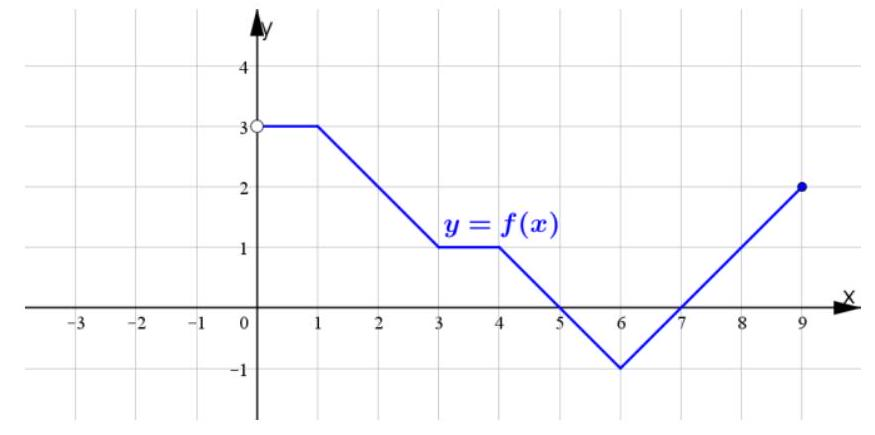
\includegraphics[max width=\textwidth, center]{2024_11_21_e75cb8afbb07ee23b21bg-10}

Zadanie 16.1. (0-1) \(\triangle B C D\)\\
Oceń prawdziwość poniższych stwierdzeń. Zaznacz P , jeśli stwierdzenie jest prawdziwe, albo \(F\) - jeśli jest falszywe.

\begin{center}
\begin{tabular}{|c|l|c|c|}
\hline
1. & Przedział \([-1 ; 3)\) jest zbiorem wszystkich wartości funkcji \(f\). & \(\mathbf{P}\) & \(\mathbf{F}\) \\
\hline
2. & Liczby 1 oraz 3 są miejscami zerowymi funkcji \(g(x)=f(x+4)\) & \(\mathbf{P}\) & \(\mathbf{F}\) \\
\hline
\end{tabular}
\end{center}

\begin{center}
\begin{tabular}{|c|c|c|c|c|c|c|c|c|c|c|c|c|c|c|c|c|c|c|c|c|c|c|c|c|}
\hline
\multicolumn{4}{|l|}{Brudnopis} &  &  &  &  &  &  &  &  &  &  &  &  &  &  &  &  &  &  &  &  &  \\
\hline
 &  &  &  &  &  &  &  &  &  &  &  &  &  &  &  &  &  &  &  &  &  &  &  &  \\
\hline
 &  &  &  &  &  &  &  &  &  &  &  &  &  &  &  &  &  &  &  &  &  &  &  &  \\
\hline
 &  &  &  &  &  &  &  &  &  &  &  &  &  &  &  &  &  &  &  &  &  &  &  &  \\
\hline
 &  &  &  &  &  &  &  &  &  &  &  &  &  &  &  &  &  &  &  &  &  &  &  &  \\
\hline
 &  &  &  &  &  &  &  &  &  &  &  &  &  &  &  &  &  &  &  &  &  &  &  &  \\
\hline
 &  &  &  &  &  &  &  &  &  &  &  &  &  &  &  &  &  &  &  &  &  &  &  &  \\
\hline
 &  &  &  &  &  &  &  &  &  &  &  &  &  &  &  &  &  &  &  &  &  &  &  &  \\
\hline
 &  &  &  &  &  &  &  &  &  &  &  &  &  &  &  &  &  &  &  &  &  &  &  &  \\
\hline
 &  &  &  &  &  &  &  &  &  &  &  &  &  &  &  &  &  &  &  &  &  &  &  &  \\
\hline
\end{tabular}
\end{center}

Zadanie 16.2 (0-1) \(\triangle\) B C C\\
Dokończ zdanie. Wybierz wlaściwą odpowiedź spośród podanych.\\
Największa wartość funkcji \(f\) w przedziale [2: 8] jest równa\\
A. 3\\
B. -1\\
C. 2\\
D. 1

\begin{center}
\begin{tabular}{|c|c|c|c|c|c|c|c|c|c|c|c|c|c|c|c|c|c|c|c|c|c|c|}
\hline
\multicolumn{4}{|l|}{Brudnopis} &  &  &  &  &  &  &  &  &  &  &  &  &  &  &  &  &  &  &  \\
\hline
 &  &  &  &  &  &  &  &  &  &  &  &  &  &  &  &  &  &  &  &  &  &  \\
\hline
 &  &  &  &  &  &  &  &  &  &  &  &  &  &  &  &  &  &  &  &  &  &  \\
\hline
 &  &  &  &  &  &  &  &  &  &  &  &  &  &  &  &  &  &  &  &  &  &  \\
\hline
 &  &  &  &  &  &  &  &  &  &  &  &  &  &  &  &  &  &  &  &  &  &  \\
\hline
 &  &  &  &  &  &  &  &  &  &  &  &  &  &  &  &  &  &  &  &  &  &  \\
\hline
 &  &  &  &  &  &  &  &  &  &  &  &  &  &  &  &  &  &  &  &  &  &  \\
\hline
 &  &  &  &  &  &  &  &  &  &  &  &  &  &  &  &  &  &  &  &  &  &  \\
\hline
 &  &  &  &  &  &  &  &  &  &  &  &  &  &  &  &  &  &  &  &  &  &  \\
\hline
 &  &  &  &  &  &  &  &  &  &  &  &  &  &  &  &  &  &  &  &  &  &  \\
\hline
 &  &  &  &  &  &  &  &  &  &  &  &  &  &  &  &  &  &  &  &  &  &  \\
\hline
\end{tabular}
\end{center}

Dokończ zdanie. Wybierz właściwą odpowiedź spośród podanych.\\
Wartość wyrażenia \(f\left(\frac{\sqrt{2}}{2}\right)-f(6)\) jest równa\\
A. \(\sqrt{2}-6\)\\
B. 2\\
C. 3\\
D. 4\\

\includegraphics[max width=\textwidth, center]{2024_11_21_e75cb8afbb07ee23b21bg-11(1)}\\
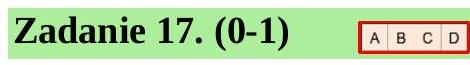
\includegraphics[max width=\textwidth, center]{2024_11_21_e75cb8afbb07ee23b21bg-11}\\
Kąt \(\alpha\) jest ostry oraz \(\sin \alpha \cdot \cos \alpha=\frac{1}{3}\).\\
Dokończ zdanie. Wybierz właściwą odpowiedź spośród podanych.\\
Wartość wyrażenia \(\frac{\sin \alpha}{\cos \alpha}+\frac{\cos \alpha}{\sin \alpha}\) jest równa\\
A. 3\\
B. 1\\
C. 2\\
D. \(\frac{1}{2}\)

\begin{center}
\begin{tabular}{|c|c|c|c|c|c|c|c|c|c|c|c|c|c|c|c|c|c|c|c|c|c|c|c|c|c|c|}
\hline
\multicolumn{5}{|l|}{Brudnopis} &  &  &  &  &  &  &  &  &  &  &  &  &  &  &  &  &  &  &  &  &  &  \\
\hline
 &  &  &  &  &  &  &  &  &  &  &  &  &  &  &  &  &  &  &  &  &  &  &  &  &  &  \\
\hline
 &  &  &  &  &  &  &  &  &  &  &  &  &  &  &  &  &  &  &  &  &  &  &  &  &  &  \\
\hline
 &  &  &  &  &  &  &  &  &  &  &  &  &  &  &  &  &  &  &  &  &  &  &  &  &  &  \\
\hline
 &  &  &  &  &  &  &  &  &  &  &  &  &  &  &  &  &  &  &  &  &  &  &  &  &  &  \\
\hline
 &  &  &  &  &  &  &  &  &  &  &  &  &  &  &  &  &  &  &  &  &  &  &  &  &  &  \\
\hline
 &  &  &  &  &  &  &  &  &  &  &  &  &  &  &  &  &  &  &  &  &  &  &  &  &  &  \\
\hline
 &  &  &  &  &  &  &  &  &  &  &  &  &  &  &  &  &  &  &  &  &  &  &  &  &  &  \\
\hline
\end{tabular}
\end{center}

Zadanie 18. (0-1) А в с D\\
Dokończ zdanie. Wybierz wlaściwą odpowiedź spośród podanych.\\
Wszystkich liczb naturalnych czterocyfrowych, w których zapisie dziesiętnym nie występują cyfry 8 i 9, jest\\
A. \(8 \cdot 8 \cdot 8 \cdot 7\)\\
B. \(6 \cdot 7 \cdot 8 \cdot 7\)\\
C. \(8 \cdot 8 \cdot 8 \cdot 8\)\\
D. \(4 \cdot 5 \cdot 6 \cdot 7\)

\begin{center}
\begin{tabular}{|c|c|c|c|c|c|c|c|c|c|c|c|c|c|c|c|c|c|c|c|c|c|c|c|c|c|c|}
\hline
\multicolumn{4}{|l|}{Brudnopis} &  &  &  &  &  &  &  &  &  &  &  &  &  &  &  &  &  &  &  &  &  &  &  \\
\hline
 &  &  &  &  &  &  &  &  &  &  &  &  &  &  &  &  &  &  &  &  &  &  &  &  &  &  \\
\hline
 &  &  &  &  &  &  &  &  &  &  &  &  &  &  &  &  &  &  &  &  &  &  &  &  &  &  \\
\hline
 &  &  &  &  &  &  &  &  &  &  &  &  &  &  &  &  &  &  &  &  &  &  &  &  &  &  \\
\hline
 &  &  &  &  &  &  &  &  &  &  &  &  &  &  &  &  &  &  &  &  &  &  &  &  &  &  \\
\hline
 &  &  &  &  &  &  &  &  &  &  &  &  &  &  &  &  &  &  &  &  &  &  &  &  &  &  \\
\hline
 &  &  &  &  &  &  &  &  &  &  &  &  &  &  &  &  &  &  &  &  &  &  &  &  &  &  \\
\hline
 &  &  &  &  &  &  &  &  &  &  &  &  &  &  &  &  &  &  &  &  &  &  &  &  &  &  \\
\hline
\end{tabular}
\end{center}

\section*{Zadanie 19.}
W grupie 100 osób przeprowadzono sondaż zadając pytanie: Ile książek przeczytałeś/przeczytałaś w 2022 roku? Wyniki sondażu przedstawiono na poniższym wykresie.\\
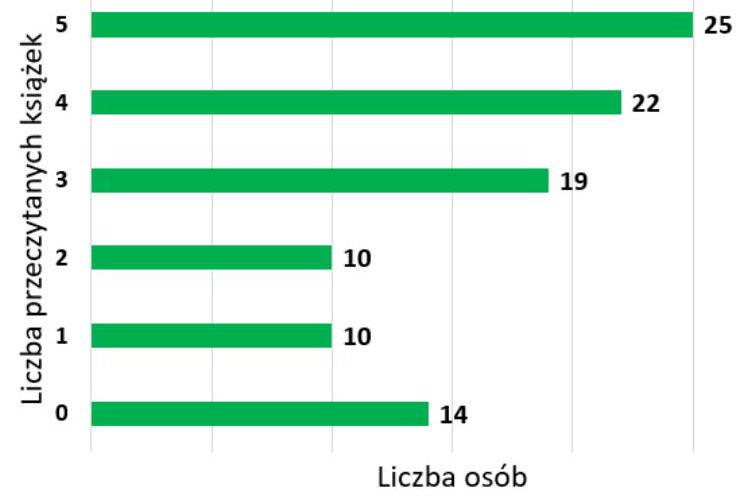
\includegraphics[max width=\textwidth, center]{2024_11_21_e75cb8afbb07ee23b21bg-12}

Zadanie 19.1. (0-1) A в с D\\
Dokończ zdanie. Wybierz właściwą odpowiedź spośród podanych.\\
Mediana liczb przeczytanych książek jest równa\\
A. 3,5\\
B. 2,5\\
C. 5\\
D. 3

\begin{center}
\begin{tabular}{|c|c|c|c|c|c|c|c|c|c|c|c|c|c|c|c|c|c|c|c|c|c|c|c|c|c|c|c|c|c|c|}
\hline
\multicolumn{5}{|l|}{Brudnopis} &  &  &  &  &  &  &  &  &  &  &  &  &  &  &  &  &  &  &  &  &  &  &  &  &  &  \\
\hline
 &  &  &  &  &  &  &  &  &  &  &  &  &  &  &  &  &  &  &  &  &  &  &  &  &  &  &  &  &  &  \\
\hline
 &  &  &  &  &  &  &  &  &  &  &  &  &  &  &  &  &  &  &  &  &  &  &  &  &  &  &  &  &  &  \\
\hline
 &  &  &  &  &  &  &  &  &  &  &  &  &  &  &  &  &  &  &  &  &  &  &  &  &  &  &  &  &  &  \\
\hline
 &  &  &  &  &  &  &  &  &  &  &  &  &  &  &  &  &  &  &  &  &  &  &  &  &  &  &  &  &  &  \\
\hline
 &  &  &  &  &  &  &  &  &  &  &  &  &  &  &  &  &  &  &  &  &  &  &  &  &  &  &  &  &  &  \\
\hline
 &  &  &  &  &  &  &  &  &  &  &  &  &  &  &  &  &  &  &  &  &  &  &  &  &  &  &  &  &  &  \\
\hline
 &  &  &  &  &  &  &  &  &  &  &  &  &  &  &  &  &  &  &  &  &  &  &  &  &  &  &  &  &  &  \\
\hline
 &  &  &  &  &  &  &  &  &  &  &  &  &  &  &  &  &  &  &  &  &  &  &  &  &  &  &  &  &  &  \\
\hline
 &  &  &  &  &  &  &  &  &  &  &  &  &  &  &  &  &  &  &  &  &  &  &  &  &  &  &  &  &  &  \\
\hline
\end{tabular}
\end{center}

Zadanie 19.2. (0-1) \(\triangle \mathrm{B}\) с D

\section*{Dokończ zdanie. Wybierz właściwą odpowiedź spośród podanych.}
Średnia arytmetyczna przeczytanych książek przez ankietowanych jest równa\\
A. 3\\
B. 3,5\\
C. 4\\
D. 2,5\\

\includegraphics[max width=\textwidth, center]{2024_11_21_e75cb8afbb07ee23b21bg-12(1)}

\section*{Zadanie 20. (0-1) A в с}
Na płaszczyźnie, w kartezjańskim układzie współrzędnych \((x, y)\), dana jest prosta \(k\) o równaniu \(y=\frac{3}{4} x+2\) oraz punkt \(A=(-2,3)\).

Dokończ zdanie. Wybierz właściwą odpowiedź spośród podanych.\\
Odległość punktu \(A\) od prostej \(k\) jest równa\\
A. 2\\
B. 3\\
C. 5\\
D. 6

\begin{center}
\begin{tabular}{|c|c|c|c|c|c|c|c|c|c|c|c|c|c|c|c|c|c|c|c|c|c|c|c|c|c|}
\hline
\multicolumn{5}{|l|}{Brudnopis} &  &  &  &  &  &  &  &  &  &  &  &  &  &  &  &  &  &  &  &  &  \\
\hline
 &  &  &  &  &  &  &  &  &  &  &  &  &  &  &  &  &  &  &  &  &  &  &  &  &  \\
\hline
 &  &  &  &  &  &  &  &  &  &  &  &  &  &  &  &  &  &  &  &  &  &  &  &  &  \\
\hline
 &  &  &  &  &  &  &  &  &  &  &  &  &  &  &  &  &  &  &  &  &  &  &  &  &  \\
\hline
 &  &  &  &  &  &  &  &  &  &  &  &  &  &  &  &  &  &  &  &  &  &  &  &  &  \\
\hline
 &  &  &  &  &  &  &  &  &  &  &  &  &  &  &  &  &  &  &  &  &  &  &  &  &  \\
\hline
 &  &  &  &  &  &  &  &  &  &  &  &  &  &  &  &  &  &  &  &  &  &  &  &  &  \\
\hline
 &  &  &  &  &  &  &  &  &  &  &  &  &  &  &  &  &  &  &  &  &  &  &  &  &  \\
\hline
 &  &  &  &  &  &  &  &  &  &  &  &  &  &  &  &  &  &  &  &  &  &  &  &  &  \\
\hline
\end{tabular}
\end{center}

\section*{Zadanie 21. (0-1) A в с D}
W trapezie prostokątnym \(A B C D\), przedstawionym na poniższym rysunku, \(|D C|=|B C|\) oraz sinus kata \(A B C\) jest równy \(\frac{4}{5}\).\\
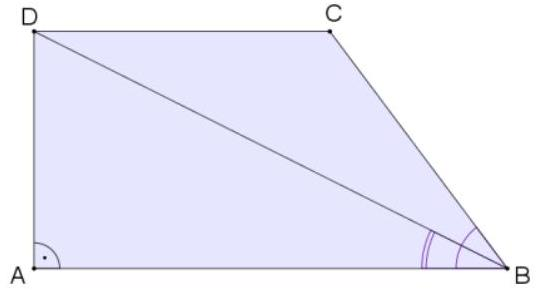
\includegraphics[max width=\textwidth, center]{2024_11_21_e75cb8afbb07ee23b21bg-13}

Dokończ zdanie. Wybierz właściwą odpowiedź spośród podanych.\\
Tangens kąta \(A B D\) jest równy\\
A. \(\frac{4}{3}\)\\
B. 0,45\\
C. \(\frac{1}{3}\)\\
D. \(\frac{1}{2}\)\\

\includegraphics[max width=\textwidth, center]{2024_11_21_e75cb8afbb07ee23b21bg-13(1)}

W trójkącie prostokątnym \(A B C\) przyprostokątna \(B C\) ma długość 8, a przeciwprostokątna \(A B\) ma długość 10. Dwusieczna kąta \(C B A\) przecina przyprostokątną \(A C\) w punkcie \(D\).

\section*{Dokończ zdanie. Wybierz właściwą odpowiedź spośród podanych.}
\begin{center}
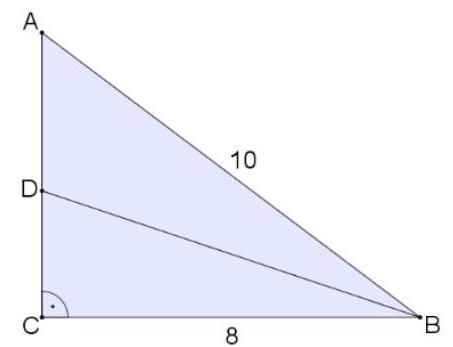
\includegraphics[max width=\textwidth]{2024_11_21_e75cb8afbb07ee23b21bg-14}
\end{center}

Długość odcinka \(C D\) jest równa\\
A. 3\\
B. \(3 \frac{1}{2}\)\\
C. \(2 \frac{2}{3}\)\\
D. 2

\begin{center}
\begin{tabular}{|c|c|c|c|c|c|c|c|c|c|c|c|c|c|c|c|c|c|c|c|c|c|c|c|c|c|c|c|}
\hline
\multicolumn{5}{|l|}{Brudnopis} &  &  &  &  &  &  &  &  &  &  &  &  &  &  &  &  &  &  &  &  &  &  &  \\
\hline
 &  &  &  &  &  &  &  &  &  &  &  &  &  &  &  &  &  &  &  &  &  &  &  &  &  &  &  \\
\hline
 &  &  &  &  &  &  &  &  &  &  &  &  &  &  &  &  &  &  &  &  &  &  &  &  &  &  &  \\
\hline
 &  &  &  &  &  &  &  &  &  &  &  &  &  &  &  &  &  &  &  &  &  &  &  &  &  &  &  \\
\hline
 &  &  &  &  &  &  &  &  &  &  &  &  &  &  &  &  &  &  &  &  &  &  &  &  &  &  &  \\
\hline
 &  &  &  &  &  &  &  &  &  &  &  &  &  &  &  &  &  &  &  &  &  &  &  &  &  &  &  \\
\hline
 &  &  &  &  &  &  &  &  &  &  &  &  &  &  &  &  &  &  &  &  &  &  &  &  &  &  &  \\
\hline
 &  &  &  &  &  &  &  &  &  &  &  &  &  &  &  &  &  &  &  &  &  &  &  &  &  &  &  \\
\hline
 &  &  &  &  &  &  &  &  &  &  &  &  &  &  &  &  &  &  &  &  &  &  &  &  &  &  &  \\
\hline
 &  &  &  &  &  &  &  &  &  &  &  &  &  &  &  &  &  &  &  &  &  &  &  &  &  &  &  \\
\hline
 &  &  &  &  &  &  &  &  &  &  &  &  &  &  &  &  &  &  &  &  &  &  &  &  &  &  &  \\
\hline
 &  &  &  &  &  &  &  &  &  &  &  &  &  &  &  &  &  &  &  &  &  &  &  &  &  &  &  \\
\hline
 &  &  &  &  &  &  &  &  &  &  &  &  &  &  &  &  &  &  &  &  &  &  &  &  &  &  &  \\
\hline
 &  &  &  &  &  &  &  &  &  &  &  &  &  &  &  &  &  &  &  &  &  &  &  &  &  &  &  \\
\hline
 &  &  &  &  &  &  &  &  &  &  &  &  &  &  &  &  &  &  &  &  &  &  &  &  &  &  &  \\
\hline
 &  &  &  &  &  &  &  &  &  &  &  &  &  &  &  &  &  &  &  &  &  &  &  &  &  &  &  \\
\hline
\end{tabular}
\end{center}

Zadanie 23. (0-1) A в с D\\
Punkty \(A, B C, D, E\) są kolejnymi wierzchołkami pięciokąta foremnego. Spośród tych punktów wybieramy losowo dwa.

\section*{Dokończ zdanie. Wybierz właściwą odpowiedź spośród podanych.}
Prawdopodobieństwo wylosowania punktów, które są końcami odcinków będących przekątnymi tego pięciokąta jest równe\\
A. \(\frac{1}{4}\)\\
B. \(\frac{1}{2}\)\\
C. \(\frac{1}{3}\)\\
D. \(\frac{3}{5}\)

\begin{center}
\begin{tabular}{|c|c|c|c|c|c|c|c|c|c|c|c|c|c|c|c|c|c|c|c|c|c|c|c|c|c|c|}
\hline
\multicolumn{5}{|l|}{Brudnopis} &  &  &  &  &  &  &  &  &  &  &  &  &  &  &  &  &  &  &  &  &  &  \\
\hline
 &  &  &  &  &  &  &  &  &  &  &  &  &  &  &  &  &  &  &  &  &  &  &  &  &  &  \\
\hline
 &  &  &  &  &  &  &  &  &  &  &  &  &  &  &  &  &  &  &  &  &  &  &  &  &  &  \\
\hline
 &  &  &  &  &  &  &  &  &  &  &  &  &  &  &  &  &  &  &  &  &  &  &  &  &  &  \\
\hline
 &  &  &  &  &  &  &  &  &  &  &  &  &  &  &  &  &  &  &  &  &  &  &  &  &  &  \\
\hline
 &  &  &  &  &  &  &  &  &  &  &  &  &  &  &  &  &  &  &  &  &  &  &  &  &  &  \\
\hline
 &  &  &  &  &  &  &  &  &  &  &  &  &  &  &  &  &  &  &  &  &  &  &  &  &  &  \\
\hline
 &  &  &  &  &  &  &  &  &  &  &  &  &  &  &  &  &  &  &  &  &  &  &  &  &  &  \\
\hline
 &  &  &  &  &  &  &  &  &  &  &  &  &  &  &  &  &  &  &  &  &  &  &  &  &  &  \\
\hline
 &  &  &  &  &  &  &  &  &  &  &  &  &  &  &  &  &  &  &  &  &  &  &  &  &  &  \\
\hline
 &  &  &  &  &  &  &  &  &  &  &  &  &  &  &  &  &  &  &  &  &  &  &  &  &  &  \\
\hline
\end{tabular}
\end{center}

\section*{Zadanie 24. (0-1) А в с D}
W kartezjańskim układzie współrzędnych \((x, y)\) przedstawiono okrąg o środku \(S=(-2,1)\). Punkt \(P=(1,1)\) leży na tym okręgu.\\
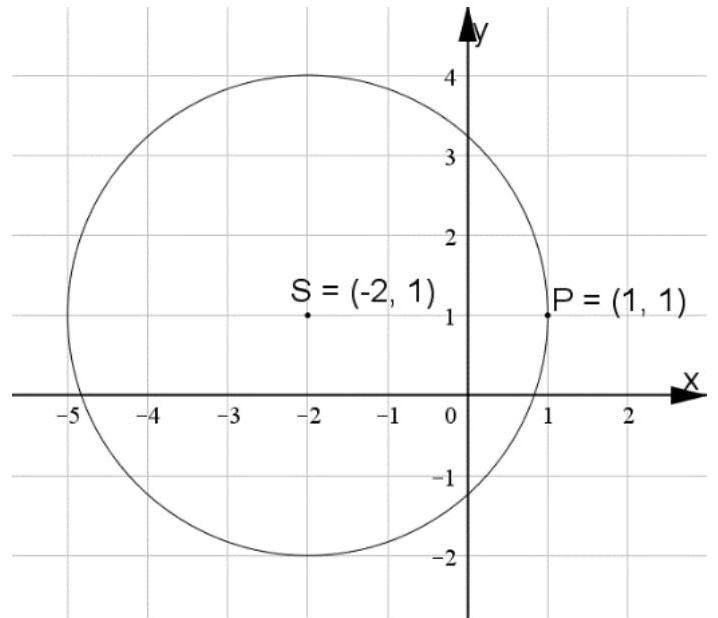
\includegraphics[max width=\textwidth, center]{2024_11_21_e75cb8afbb07ee23b21bg-15(1)}

Dokończ zdanie. Wybierz właściwą odpowiedź spośród podanych.\\
Równanie okręgu przedstawionego na rysunku ma postać\\
A. \((x-2)^{2}+(y+1)^{2}=3\)\\
B. \((x+2)^{2}+(y-1)^{2}=3\)\\
C. \((x-2)^{2}+(y+1)^{2}=9\)\\
D. \((x+2)^{2}+(y-1)^{2}=9\)

\begin{center}
\begin{tabular}{|c|c|c|c|c|c|c|c|c|c|c|c|c|c|c|c|c|c|c|c|c|c|c|c|c|c|c|}
\hline
\multicolumn{4}{|l|}{Brudnopis} &  &  &  &  &  &  &  &  &  &  &  &  &  &  &  &  &  &  &  &  &  &  &  \\
\hline
 &  &  &  &  &  &  &  &  &  &  &  &  &  &  &  &  &  &  &  &  &  &  &  &  &  &  \\
\hline
 &  &  &  &  &  &  &  &  &  &  &  &  &  &  &  &  &  &  &  &  &  &  &  &  &  &  \\
\hline
 &  &  &  &  &  &  &  &  &  &  &  &  &  &  &  &  &  &  &  &  &  &  &  &  &  &  \\
\hline
 &  &  &  &  &  &  &  &  &  &  &  &  &  &  &  &  &  &  &  &  &  &  &  &  &  &  \\
\hline
 &  &  &  &  &  &  &  &  &  &  &  &  &  &  &  &  &  &  &  &  &  &  &  &  &  &  \\
\hline
\end{tabular}
\end{center}

Zadanie 25. (0-1) A в с D\\
Prosta \(l\) jest styczna w punkcie \(P\) do okręgu o środku \(O\) (zobacz rysunek). Prosta \(k\) przechodząca przez punkt \(O\) przecina prostą \(l\) w punkcie \(A\). Prosta \(m\) przechodzi przez punkt \(A\) oraz jest prostopadła do prostej \(k\). Miara kąta \(P O A\) jest równa \(61^{\circ}\).\\
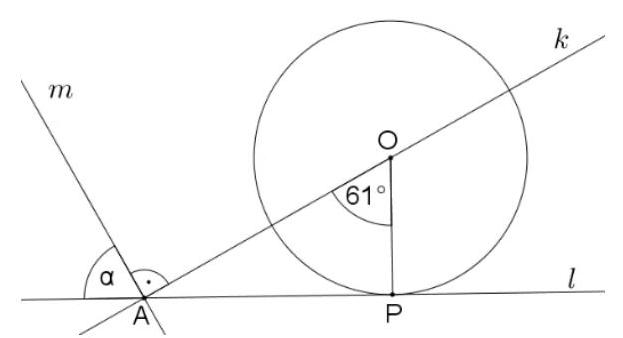
\includegraphics[max width=\textwidth, center]{2024_11_21_e75cb8afbb07ee23b21bg-15}

\section*{Dokończ zdanie. Wybierz wlaściwą odpowiedź spośród podanych.}
Miara kąta \(\alpha\) jest równa\\
A. \(59^{\circ}\)\\
B. \(29^{\circ}\)\\
C. \(61^{\circ}\)\\
D. \(79^{\circ}\)\\

\includegraphics[max width=\textwidth, center]{2024_11_21_e75cb8afbb07ee23b21bg-15(2)}

Odcinki \(A B\) i \(D E\) są równoległe. Długości odcinków \(A B\) i \(D E\) są odpowiednio równe 20 i 4. Pole trójkąta \(D E C\) jest równe 5. Oblicz pole trapezu \(A B D E\).\\
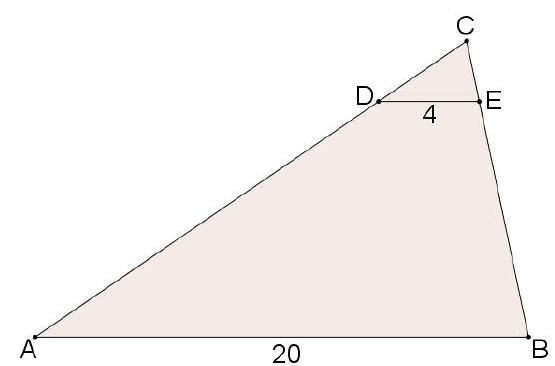
\includegraphics[max width=\textwidth, center]{2024_11_21_e75cb8afbb07ee23b21bg-16}

\section*{Zapisz obliczenia}
\begin{center}

\includegraphics[max width=\textwidth]{2024_11_21_e75cb8afbb07ee23b21bg-16(1)}
\end{center}

Dany jest trójkąt \(A B C\), w którym \(|A B|=29,|A C|=26\) oraz sinus kąta ostrego \(B A C\) jest równy \(\frac{5}{13}\).\\
Oblicz długość boku \(B C\).

\section*{Zapisz obliczenia.}
\begin{center}
\begin{tabular}{|c|c|c|c|c|c|c|c|c|c|c|c|c|c|c|c|c|c|c|c|c|c|}
\hline
 &  &  &  &  &  &  &  &  &  &  &  &  &  &  &  &  &  &  &  &  &  \\
\hline
 &  &  &  &  &  &  &  &  &  &  &  &  &  &  &  &  &  &  &  &  &  \\
\hline
 &  &  &  &  &  &  &  &  &  &  &  &  &  &  &  &  &  &  &  &  &  \\
\hline
 &  &  &  &  &  &  &  &  &  &  &  &  &  &  &  &  &  &  &  &  &  \\
\hline
 &  &  &  &  &  &  &  &  &  &  &  &  &  &  &  &  &  &  &  &  &  \\
\hline
 &  &  &  &  &  &  &  &  &  &  &  &  &  &  &  &  &  &  &  &  &  \\
\hline
 &  &  &  &  &  &  &  &  &  &  &  &  &  &  &  &  &  &  &  &  &  \\
\hline
 &  &  &  &  &  &  &  &  &  &  &  &  &  &  &  &  &  &  &  &  &  \\
\hline
 &  &  &  &  &  &  &  &  &  &  &  &  &  &  &  &  &  &  &  &  &  \\
\hline
 &  &  &  &  &  &  &  &  &  &  &  &  &  &  &  &  &  &  &  &  &  \\
\hline
 &  &  &  &  &  &  &  &  &  &  &  &  &  &  &  &  &  &  &  &  &  \\
\hline
 &  &  &  &  &  &  &  &  &  &  &  &  &  &  &  &  &  &  &  &  &  \\
\hline
 &  &  &  &  &  &  &  &  &  &  &  &  &  &  &  &  &  &  &  &  &  \\
\hline
 &  &  &  &  &  &  &  &  &  &  &  &  &  &  &  &  &  &  &  &  &  \\
\hline
 &  &  &  &  &  &  &  &  &  &  &  &  &  &  &  &  &  &  &  &  &  \\
\hline
 &  &  &  &  &  &  &  &  &  &  &  &  &  &  &  &  &  &  &  &  &  \\
\hline
 &  &  &  &  &  &  &  &  &  &  &  &  &  &  &  &  &  &  &  &  &  \\
\hline
 &  &  &  &  &  &  &  &  &  &  &  &  &  &  &  &  &  &  &  &  &  \\
\hline
 &  &  &  &  &  &  &  &  &  &  &  &  &  &  &  &  &  &  &  &  &  \\
\hline
 &  &  &  &  &  &  &  &  &  &  &  &  &  &  &  &  &  &  &  &  &  \\
\hline
 &  &  &  &  &  &  &  &  &  &  &  &  &  &  &  &  &  &  &  &  &  \\
\hline
 &  &  &  &  &  &  &  &  &  &  &  &  &  &  &  &  &  &  &  &  &  \\
\hline
 &  &  &  &  &  &  &  &  &  &  &  &  &  &  &  &  &  &  &  &  &  \\
\hline
 &  &  &  &  &  &  &  &  &  &  &  &  &  &  &  &  &  &  &  &  &  \\
\hline
 &  &  &  &  &  &  &  &  &  &  &  &  &  &  &  &  &  &  &  &  &  \\
\hline
 &  &  &  &  &  &  &  &  &  &  &  &  &  &  &  &  &  &  &  &  &  \\
\hline
 &  &  &  &  &  &  &  &  &  &  &  &  &  &  &  &  &  &  &  &  &  \\
\hline
 &  &  &  &  &  &  &  &  &  &  &  &  &  &  &  &  &  &  &  &  &  \\
\hline
 &  &  &  &  &  &  &  &  &  &  &  &  &  &  &  &  &  &  &  &  &  \\
\hline
 &  &  &  &  &  &  &  &  &  &  &  &  &  &  &  &  &  &  &  &  &  \\
\hline
 &  &  &  &  &  &  &  &  &  &  &  &  &  &  &  &  &  &  &  &  &  \\
\hline
 &  &  &  &  &  &  &  &  &  &  &  &  &  &  &  &  &  &  &  &  &  \\
\hline
 &  &  &  &  &  &  &  &  &  &  &  &  &  &  &  &  &  &  &  &  &  \\
\hline
 &  &  &  &  &  &  &  &  &  &  &  &  &  &  &  &  &  &  &  &  &  \\
\hline
 &  &  &  &  &  &  &  &  &  &  &  &  &  &  &  &  &  &  &  &  &  \\
\hline
 &  &  &  &  &  &  &  &  &  &  &  &  &  &  &  &  &  &  &  &  &  \\
\hline
 &  &  &  &  &  &  &  &  &  &  &  &  &  &  &  &  &  &  &  &  &  \\
\hline
 &  &  &  &  &  &  &  &  &  &  &  &  &  &  &  &  &  &  &  &  &  \\
\hline
\end{tabular}
\end{center}

Wysokość ostrosłupa prawidłowego trójkątnego jest równa 8 a pole jego podstawy wynosi \(27 \sqrt{3}\). Oblicz długość krawędzi bocznej tego ostrosłupa.

\section*{Zapisz obliczenia.}
\begin{center}
\begin{tabular}{|c|c|c|c|c|c|c|c|c|c|c|c|c|c|c|c|c|c|c|c|c|c|c|c|c|c|c|}
\hline
 &  &  &  &  &  &  &  &  &  &  &  &  &  &  &  &  &  &  &  &  &  &  &  &  &  &  \\
\hline
 &  &  &  &  &  &  &  &  &  &  &  &  &  &  &  &  &  &  &  &  &  &  &  &  &  &  \\
\hline
 &  &  &  &  &  &  &  &  &  &  &  &  &  &  &  &  &  &  &  &  &  &  &  &  &  &  \\
\hline
 &  &  &  &  &  &  &  &  &  &  &  &  &  &  &  &  &  &  &  &  &  &  &  &  &  &  \\
\hline
 &  &  &  &  &  &  &  &  &  &  &  &  &  &  &  &  &  &  &  &  &  &  &  &  &  &  \\
\hline
 &  &  &  &  &  &  &  &  &  &  &  &  &  &  &  &  &  &  &  &  &  &  &  &  &  &  \\
\hline
 &  &  &  &  &  &  &  &  &  &  &  &  &  &  &  &  &  &  &  &  &  &  &  &  &  &  \\
\hline
 &  &  &  &  &  &  &  &  &  &  &  &  &  &  &  &  &  &  &  &  &  &  &  &  &  &  \\
\hline
 &  &  &  &  &  &  &  &  &  &  &  &  &  &  &  &  &  &  &  &  &  &  &  &  &  &  \\
\hline
 &  &  &  &  &  &  &  &  &  &  &  &  &  &  &  &  &  &  &  &  &  &  &  &  &  &  \\
\hline
 &  &  &  &  &  &  &  &  &  &  &  &  &  &  &  &  &  &  &  &  &  &  &  &  &  &  \\
\hline
 &  &  &  &  &  &  &  &  &  &  &  &  &  &  &  &  &  &  &  &  &  &  &  &  &  &  \\
\hline
 &  &  &  &  &  &  &  &  &  &  &  &  &  &  &  &  &  &  &  &  &  &  &  &  &  &  \\
\hline
 &  &  &  &  &  &  &  &  &  &  &  &  &  &  &  &  &  &  &  &  &  &  &  &  &  &  \\
\hline
 &  &  &  &  &  &  &  &  &  &  &  &  &  &  &  &  &  &  &  &  &  &  &  &  &  &  \\
\hline
 &  &  &  &  &  &  &  &  &  &  &  &  &  &  &  &  &  &  &  &  &  &  &  &  &  &  \\
\hline
 &  &  &  &  &  &  &  &  &  &  &  &  &  &  &  &  &  &  &  &  &  &  &  &  &  &  \\
\hline
 &  &  &  &  &  &  &  &  &  &  &  &  &  &  &  &  &  &  &  &  &  &  &  &  &  &  \\
\hline
 &  &  &  &  &  &  &  &  &  &  &  &  &  &  &  &  &  &  &  &  &  &  &  &  &  &  \\
\hline
 &  &  &  &  &  &  &  &  &  &  &  &  &  &  &  &  &  &  &  &  &  &  &  &  &  &  \\
\hline
 &  &  &  &  &  &  &  &  &  &  &  &  &  &  &  &  &  &  &  &  &  &  &  &  &  &  \\
\hline
 &  &  &  &  &  &  &  &  &  &  &  &  &  &  &  &  &  &  &  &  &  &  &  &  &  &  \\
\hline
 &  &  &  &  &  &  &  &  &  &  &  &  &  &  &  &  &  &  &  &  &  &  &  &  &  &  \\
\hline
 &  &  &  &  &  &  &  &  &  &  &  &  &  &  &  &  &  &  &  &  &  &  &  &  &  &  \\
\hline
 &  &  &  &  &  &  &  &  &  &  &  &  &  &  &  &  &  &  &  &  &  &  &  &  &  &  \\
\hline
 &  &  &  &  &  &  &  &  &  &  &  &  &  &  &  &  &  &  &  &  &  &  &  &  &  &  \\
\hline
 &  &  &  &  &  &  &  &  &  &  &  &  &  &  &  &  &  &  &  &  &  &  &  &  &  &  \\
\hline
 &  &  &  &  &  &  &  &  &  &  &  &  &  &  &  &  &  &  &  &  &  &  &  &  &  &  \\
\hline
 &  &  &  &  &  &  &  &  &  &  &  &  &  &  &  &  &  &  &  &  &  &  &  &  &  &  \\
\hline
 &  &  &  &  &  &  &  &  &  &  &  &  &  &  &  &  &  &  &  &  &  &  &  &  &  &  \\
\hline
 &  &  &  &  &  &  &  &  &  &  &  &  &  &  &  &  &  &  &  &  &  &  &  &  &  &  \\
\hline
 &  &  &  &  &  &  &  &  &  &  &  &  &  &  &  &  &  &  &  &  &  &  &  &  &  &  \\
\hline
 &  &  &  &  &  &  &  &  &  &  &  &  &  &  &  &  &  &  &  &  &  &  &  &  &  &  \\
\hline
 &  &  &  &  &  &  &  &  &  &  &  &  &  &  &  &  &  &  &  &  &  &  &  &  &  &  \\
\hline
 &  &  &  &  &  &  &  &  &  &  &  &  &  &  &  &  &  &  &  &  &  &  &  &  &  &  \\
\hline
 &  &  &  &  &  &  &  &  &  &  &  &  &  &  &  &  &  &  &  &  &  &  &  &  &  &  \\
\hline
 &  &  &  &  &  &  &  &  &  &  &  &  &  &  &  &  &  &  &  &  &  &  &  &  &  &  \\
\hline
 &  &  &  &  &  &  &  &  &  &  &  &  &  &  &  &  &  &  &  &  &  &  &  &  &  &  \\
\hline
 &  &  &  &  &  &  &  &  &  &  &  &  &  &  &  &  &  &  &  &  &  &  &  &  &  &  \\
\hline
\end{tabular}
\end{center}

Podstawą graniastosłupa prostego jest prostokąt, w którym stosunek długości jego boków jest równy 1:2. Suma długości trzech krawędzi wychodzących z jednego wierzchołka jest równa 14. Wyznacz wymiary graniastosłupa, którego pole powierzchni całkowitej jest największe.

Zapisz obliczenia.

\begin{center}
\begin{tabular}{|c|c|c|c|c|c|c|c|c|c|c|c|c|c|c|c|c|c|c|c|c|c|c|c|}
\hline
 &  &  &  &  &  &  &  &  &  &  &  &  &  &  &  &  &  &  &  &  &  &  &  \\
\hline
 &  &  &  &  &  &  &  &  &  &  &  &  &  &  &  &  &  &  &  &  &  &  &  \\
\hline
 &  &  &  &  &  &  &  &  &  &  &  &  &  &  &  &  &  &  &  &  &  &  &  \\
\hline
 &  &  &  &  &  &  &  &  &  &  &  &  &  &  &  &  &  &  &  &  &  &  &  \\
\hline
 &  &  &  &  &  &  &  &  &  &  &  &  &  &  &  &  &  &  &  &  &  &  &  \\
\hline
 &  &  &  &  &  &  &  &  &  &  &  &  &  &  &  &  &  &  &  &  &  &  &  \\
\hline
 &  &  &  &  &  &  &  &  &  &  &  &  &  &  &  &  &  &  &  &  &  &  &  \\
\hline
 &  &  &  &  &  &  &  &  &  &  &  &  &  &  &  &  &  &  &  &  &  &  &  \\
\hline
 &  &  &  &  &  &  &  &  &  &  &  &  &  &  &  &  &  &  &  &  &  &  &  \\
\hline
 &  &  &  &  &  &  &  &  &  &  &  &  &  &  &  &  &  &  &  &  &  &  &  \\
\hline
 &  &  &  &  &  &  &  &  &  &  &  &  &  &  &  &  &  &  &  &  &  &  &  \\
\hline
 &  &  &  &  &  &  &  &  &  &  &  &  &  &  &  &  &  &  &  &  &  &  &  \\
\hline
 &  &  &  &  &  &  &  &  &  &  &  &  &  &  &  &  &  &  &  &  &  &  &  \\
\hline
 &  &  &  &  &  &  &  &  &  &  &  &  &  &  &  &  &  &  &  &  &  &  &  \\
\hline
 &  &  &  &  &  &  &  &  &  &  &  &  &  &  &  &  &  &  &  &  &  &  &  \\
\hline
 &  &  &  &  &  &  &  &  &  &  &  &  &  &  &  &  &  &  &  &  &  &  &  \\
\hline
 &  &  &  &  &  &  &  &  &  &  &  &  &  &  &  &  &  &  &  &  &  &  &  \\
\hline
 &  &  &  &  &  &  &  &  &  &  &  &  &  &  &  &  &  &  &  &  &  &  &  \\
\hline
 &  &  &  &  &  &  &  &  &  &  &  &  &  &  &  &  &  &  &  &  &  &  &  \\
\hline
 &  &  &  &  &  &  &  &  &  &  &  &  &  &  &  &  &  &  &  &  &  &  &  \\
\hline
 &  &  &  &  &  &  &  &  &  &  &  &  &  &  &  &  &  &  &  &  &  &  &  \\
\hline
 &  &  &  &  &  &  &  &  &  &  &  &  &  &  &  &  &  &  &  &  &  &  &  \\
\hline
 &  &  &  &  &  &  &  &  &  &  &  &  &  &  &  &  &  &  &  &  &  &  &  \\
\hline
 &  &  &  &  &  &  &  &  &  &  &  &  &  &  &  &  &  &  &  &  &  &  &  \\
\hline
 &  &  &  &  &  &  &  &  &  &  &  &  &  &  &  &  &  &  &  &  &  &  &  \\
\hline
 &  &  &  &  &  &  &  &  &  &  &  &  &  &  &  &  &  &  &  &  &  &  &  \\
\hline
 &  &  &  &  &  &  &  &  &  &  &  &  &  &  &  &  &  &  &  &  &  &  &  \\
\hline
 &  &  &  &  &  &  &  &  &  &  &  &  &  &  &  &  &  &  &  &  &  &  &  \\
\hline
 &  &  &  &  &  &  &  &  &  &  &  &  &  &  &  &  &  &  &  &  &  &  &  \\
\hline
 &  &  &  &  &  &  &  &  &  &  &  &  &  &  &  &  &  &  &  &  &  &  &  \\
\hline
 &  &  &  &  &  &  &  &  &  &  &  &  &  &  &  &  &  &  &  &  &  &  &  \\
\hline
 &  &  &  &  &  &  &  &  &  &  &  &  &  &  &  &  &  &  &  &  &  &  &  \\
\hline
 &  &  &  &  &  &  &  &  &  &  &  &  &  &  &  &  &  &  &  &  &  &  &  \\
\hline
 &  &  &  &  &  &  &  &  &  &  &  &  &  &  &  &  &  &  &  &  &  &  &  \\
\hline
 &  &  &  &  &  &  &  &  &  &  &  &  &  &  &  &  &  &  &  &  &  &  &  \\
\hline
 &  &  &  &  &  &  &  &  &  &  &  &  &  &  &  &  &  &  &  &  &  &  &  \\
\hline
 &  &  &  &  &  &  &  &  &  &  &  &  &  &  &  &  &  &  &  &  &  &  &  \\
\hline
 &  &  &  &  &  &  &  &  &  &  &  &  &  &  &  &  &  &  &  &  &  &  &  \\
\hline
\end{tabular}
\end{center}

BRUNOPIS\\

\includegraphics[max width=\textwidth, center]{2024_11_21_e75cb8afbb07ee23b21bg-20}\\
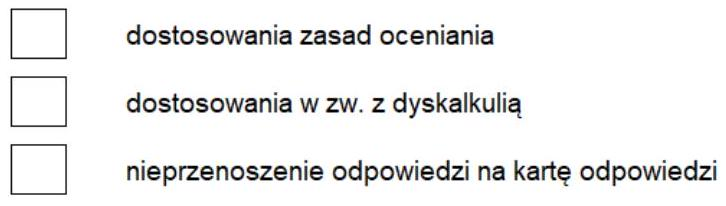
\includegraphics[max width=\textwidth, center]{2024_11_21_e75cb8afbb07ee23b21bg-21}

\section*{PESEL}
\section*{WYPEŁNIA ZDAJĄCY}
\begin{center}
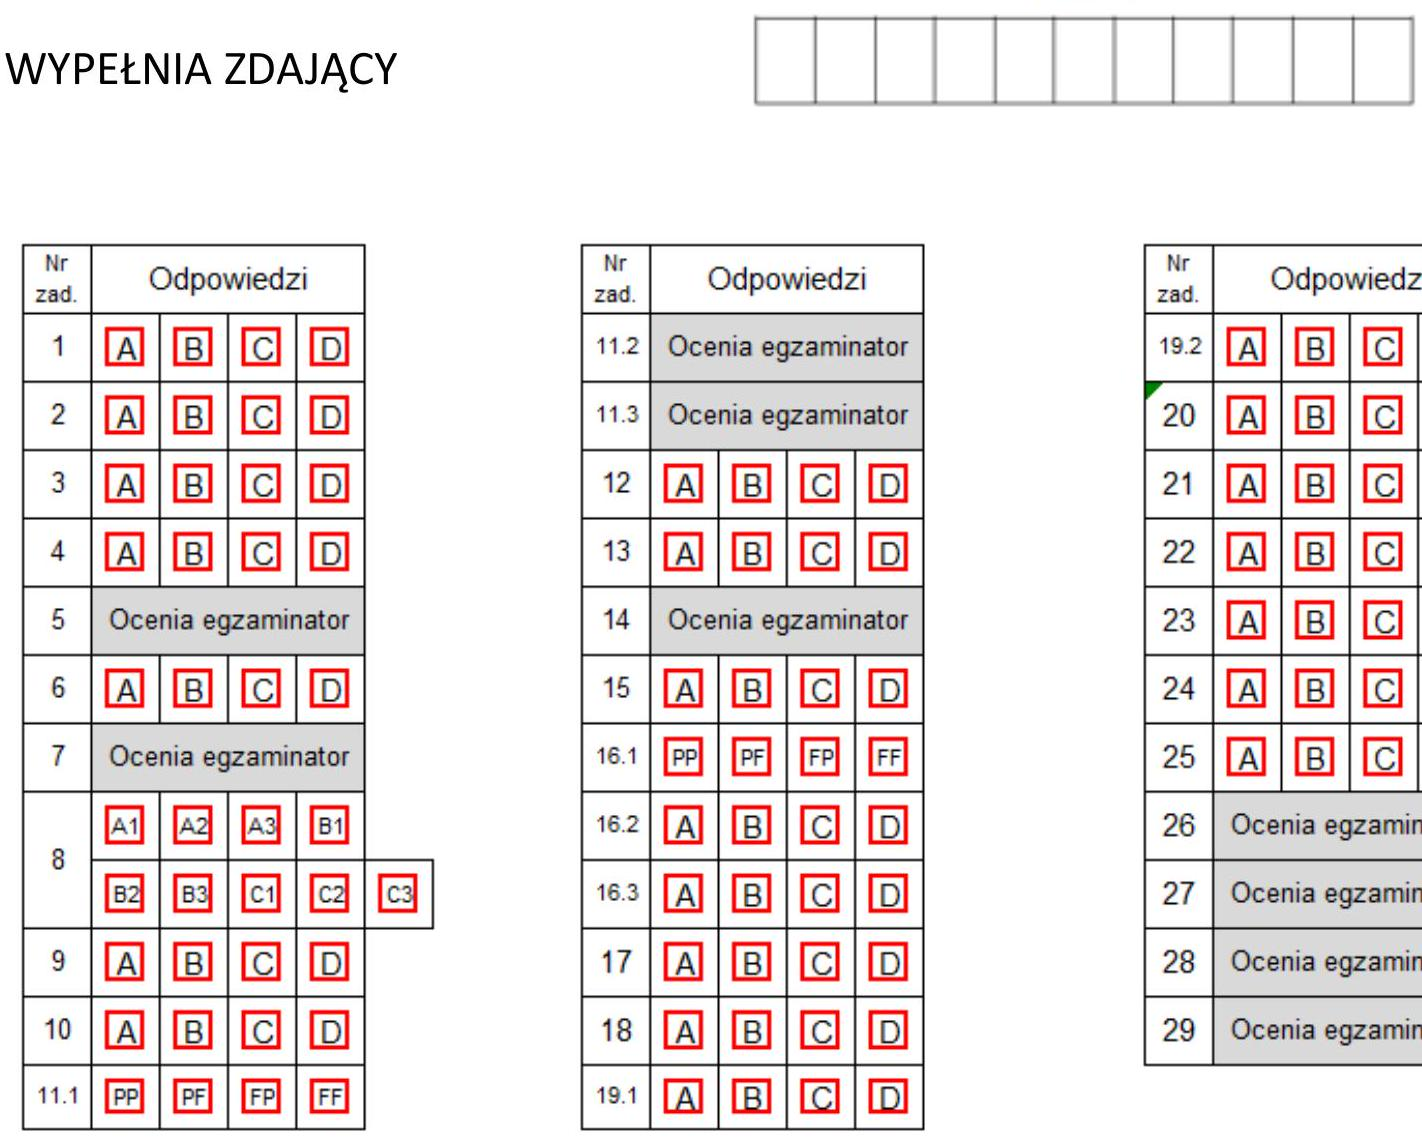
\includegraphics[max width=\textwidth]{2024_11_21_e75cb8afbb07ee23b21bg-21(2)}
\end{center}

\begin{center}
\begin{tabular}{|c|c|c|c|c|}
\hline
\begin{tabular}{c}
Nr \\
zad. \\
\end{tabular} & \multicolumn{3}{|c|}{Odpowiedzi} &  \\
\hline
19.2 & A & B & C & D \\
\hline
20 & A & B & C & D \\
\hline
21 & A & B & C & D \\
\hline
22 & A & B & C & D \\
\hline
23 & A & B & C & D \\
\hline
24 & A & B & C & D \\
\hline
25 & A & B & C & D \\
\hline
26 & Ocenia egzaminator &  &  &  \\
\hline
27 & Ocenia egzaminator &  &  &  \\
\hline
28 & Ocenia egzaminator &  &  &  \\
\hline
29 & \multicolumn{4}{|c|}{Ocenia egzaminator} \\
\hline
\end{tabular}
\end{center}

\section*{WYPEŁNIA EGZAMINATOR}
\begin{center}
\begin{tabular}{|c|c|c|c|c|}
\hline
\begin{tabular}{c}
Nr \\
zad. \\
\end{tabular} & \multicolumn{3}{|c|}{Odpowiedzi} \\
\hline
5 & 0 & 1 & 2 \\
\hline
7 & 0 & 1 & 2 \\
\hline
11.2 & 0 & 1 &  \\
\hline
\end{tabular}
\end{center}

\begin{center}
\begin{tabular}{|c|c|c|c|c|}
\hline
\begin{tabular}{c}
N \\
zad. \\
\end{tabular} & \multicolumn{4}{|c|}{Odpowiedzi} \\
\hline
11.3 & 0 & 1 & 2 &  \\
\hline
14 & 0 & 1 & 2 &  \\
\hline
26 & 0 & 1 & 2 & 3 \\
\hline
\end{tabular}
\end{center}

\begin{center}
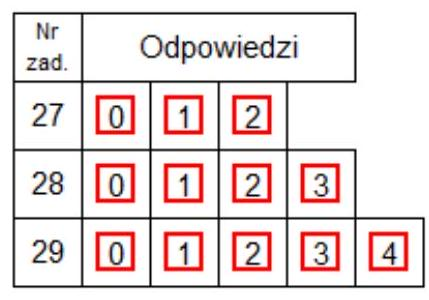
\includegraphics[max width=\textwidth]{2024_11_21_e75cb8afbb07ee23b21bg-21(1)}
\end{center}


\end{document}